% Template for a Computer Science Tripos Part II project dissertation
\documentclass[12pt,a4paper,twoside,openright]{report}
\usepackage[pdfborder={0 0 0}]{hyperref}    % turns references into hyperlinks
\usepackage[margin=25mm]{geometry}  % adjusts page layout
\usepackage{graphicx}  % allows inclusion of PDF, PNG and JPG images
\usepackage{pmboxdraw}
\usepackage{verbatim}
\usepackage{docmute}   % only needed to allow inclusion of proposal.tex
\usepackage{parskip}
\usepackage{pdfpages}
\usepackage{listings}
\usepackage{amsmath}
\usepackage{amsfonts}

\usepackage{todonotes} % remove


\lstset{basicstyle=\ttfamily, breaklines=true}

\graphicspath{ {./images/} }

\newcommand{\quickwordcount}[1]{%
  \immediate\write18{texcount -1 -sum -merge -q #1.tex output.bbl > #1-words.sum }%
  \input{#1-words.sum} words%
}

\raggedbottom                           % try to avoid widows and orphans
\sloppy
\clubpenalty1000%
\widowpenalty1000%

\renewcommand{\baselinestretch}{1.1}    % adjust line spacing to make
                                        % more readable

\begin{document}

\bibliographystyle{plain}


%%%%%%%%%%%%%%%%%%%%%%%%%%%%%%%%%%%%%%%%%%%%%%%%%%%%%%%%%%%%%%%%%%%%%%%%
% Title


\pagestyle{empty}

\rightline{\LARGE \textbf{Jiaxin Wang}}

\vspace*{60mm}
\begin{center}
\Huge
\textbf{A Recursive Recurrent Neural Network Decoder for Grammatical Error Correction} \\[5mm]
Computer Science Tripos -- Part II \\[5mm]
Emmanuel College \\[5mm]
\today  % today's date
\end{center}

%%%%%%%%%%%%%%%%%%%%%%%%%%%%%%%%%%%%%%%%%%%%%%%%%%%%%%%%%%%%%%%%%%%%%%%%%%%%%%
% Proforma, table of contents and list of figures

\pagestyle{plain}

\newpage

\section*{Declaration}

I, Jiaxin Wang of Emmanuel College, being a candidate for Part II of the Computer
Science Tripos, hereby declare that this dissertation and the work described in 
it are my own work, unaided except as may be specified below, and that the dissertation
does not contain material that has already been used to any substantial
extent for a comparable purpose.

\bigskip
\leftline{Signed [signature]}

\medskip
\leftline{Date [date]}

\chapter*{Proforma}

{\large
\begin{tabular}{ll}
Candidate Number:   & -                       \\
Project Title:      & A Recursive Recurrent Neural Network \\
 & Decoder for Grammatical Error Correction \\
Examination:        & Computer Science Tripos -- Part II, 2022  \\
Word Count:         & \quickwordcount{diss}\footnotemark[1] \\
Code line count:    & 1136 \footnotemark[2]\\
Project Originator: & - \\
Supervisor:         & Dr Zheng Yuan, Dr Christopher Bryant
\end{tabular}
}
\footnotetext[1]{This word count was computed by 
\texttt{\textbackslash immediate\textbackslash write18\{texcount -1 -sum -merge -q diss.tex output.bbl > diss-words.sum\} and \textbackslash input\{diss-words.sum\} words}}

\footnotetext[2]{Code line count was computed
by \texttt{find ./model ./helper\_scripts -name "*.py" -print | xargs wc -l}
}
\stepcounter{footnote}

\section*{Original Aims of the Project}
This project aims to build an SMT system for grammatical error correction using a recursive recurrent neural network (R\textsuperscript{2}NN) model as the decoder. It involves constructing phrase pair embedding (TCBPPE) using a feedforward neural network (FNN) and a recurrent neural network (RNN), implementing the R\textsuperscript{2}NN model and training the R\textsuperscript{2}NN SMT system. A baseline SMT system (Moses) will be built and trained with the same data. The R\textsuperscript{2}NN SMT will be evaluated against baseline SMT on the grammatical error correction task using the $F_{0.5}$ metric.

\section*{Work Completed}
All the core goals of the project have been achieved. Two SMT systems were built, namely Moses SMT and R\textsuperscript{2}NN SMT. For Moses SMT, a baseline phrase-based SMT system was constructed. For R\textsuperscript{2}NN SMT, the recursive recurrent neural network was implemented from scratch and the phrase pair embedding (TCBPPE) was obtained to be used with R\textsuperscript{2}NN. Both systems were trained and tested with the same data. Finally, a comparison was carried out on the evaluation results of the two SMT systems for the task of grammatical error correction.

\newpage

\section*{Special Difficulties}
None.

\section*{Acknowledgements}


\tableofcontents

\listoffigures

% \listoftodos

%%%%%%%%%%%%%%%%%%%%%%%%%%%%%%%%%%%%%%%%%%%%%%%%%%%%%%%%%%%%%%%%%%%%%%%
% now for the chapters

\pagestyle{headings}

\chapter{Introduction}

\section{Motivation}

Grammatical Error Correction (GEC) is the task of producing a grammatically correct sentence given a potentially erroneous text while preserving its meaning. One of the many motivations behind this task is that it plays a significant role in helping learners of a foreign language understand the language better. Being an ESL (English as a second language) learner myself, it is often difficult for me to spot the errors in my English writing since the English grammar is quite different from that of my first language. Native English speakers may wish to use a GEC system to avoid mistakes in their writing, especially in a professional environment (e.g. work emails). 

One common approach to GEC, SMT-based GEC, is to treat GEC as a translation problem and use a statistical machine translation (SMT) system to solve it. We train an SMT system that takes an erroneous source sentence as input and the grammatically correct sentence as the expected output. By searching for the best "translation" from the source sentence, the aim is to find a grammatically correct sentence that preserves the meaning of the original sentence.

Liu et al. proposed a novel model for SMT called \textit{recursive recurrent neural network} (R\textsuperscript{2}NN)\cite{r2nn}. It has a tree structure similar to recursive neural network, with recurrent input vectors to encode global information that cannot be generated by the child node representations. In the paper, they showed that the R\textsuperscript{2}NN SMT achieved better performance than a state-of-the-art baseline system on a Chinese-to-English translation task. However, they did not publicised their code, and no implementation of such R\textsuperscript{2}NN can be found on the Internet.

It is therefore of interest to implement such a neural network and apply it to the task of GEC. For one, publishing the code could benefit other researchers in this area who are interested in NLP (natural language processing), GEC, and neural networks. For another, if the R\textsuperscript{2}NN model is proven to be useful for GEC, it could help with developing better GEC systems and assist millions of English learners.

\section{Problem Overview}

An SMT system has four components: a language model (LM) which computes the probability of a given word sequence being valid, a translation model (TM) which constructs mappings of phrases between source and target corpora and calculates translation probabilities, a reordering model (RM) which handles phrase reordering, and a decoder which looks for the best translation candidate\cite{yuan2017phd}. The R\textsuperscript{2}NN model proposed by Liu et al. was used in the end-to-end decoding process of SMT, i.e. as a decoder. The goal of this project is to implement such a decoder, integrate it into an SMT system, apply it to GEC task and evaluate its performance against a baseline SMT system. 

The GEC system should aim to correct all types of errors in non-native English text specified in the BEA 2019 Shared Task\cite{bryant-etal-2019-bea}, namely grammatical, lexical and orthographic errors. Lexical errors are mistakes at word level, such as wrong choice of words that do not fit in their context. Grammatical errors violate the grammar of a certain language. Orthographic errors refer to incorrect spelling of words. 

Moses\cite{moses} will be used as the baseline SMT system to be evaluated against the R\textsuperscript{2}NN SMT. Moses is a toolkit commonly used for statistical machine translation. The toolkit contains a decoder (Moses decoder) and various tools for training and tuning. It also provides a user guide on how to use the decoder together with other models to build a SMT system. For this project, I will build and train a Moses SMT system. I will implement and train an R\textsuperscript{2}NN SMT system which uses the R\textsuperscript{2}NN model as the decoder. Finally, I will compare the performance of both systems on the task of grammatical error correction.

\section{Related Work}

The paper\cite{r2nn} by Liu et al. discussed the structure of R\textsuperscript{2}NN and how it can be used as a decoder.  They also proposed a way to initialise the phrase pair embedding called \textit{translation confidence based phrase pair embedding} (TCBPPE) to generate the leaf nodes. After training the system on data from the IWSLT 2009 dialog task, they tested the system on a Chinese-to-English translation task. Finally, they evaluated their system against a baseline decoder using the case insensitive IBM BLEU-4 method. Details of R\textsuperscript{2}NN and TCBPPE are discussed in the following chapters.

SMT systems have been successfully used for the task of grammatical error correction. Yuan and Felice\cite{yuan-felice-2013-constrained} applied Moses SMT with GIZA++ and IRSTLM to grammatical error correction in the CoNLL-2013 Shared Task\cite{ng-etal-2013-conll}. Junczys-Dowmunt and Grundkiewicz\cite{junczys-dowmunt-grundkiewicz-2014-amu} developed a GEC system based on an SMT system, namely phrase-based Moses\cite{moses}, and they ranked on the third place in the CoNLL-2014 Shared Task\cite{ng-etal-2014-conll}. Yuan et al.\cite{yuan-etal-2016-candidate} discussed how SMT can be applied to GEC and how a re-ranking model can improve the performance of SMT-based GEC system.

This project aims to implement the R\textsuperscript{2}NN together with TCBPPE in the paper\cite{r2nn} and build a SMT system. A phrase-based Moses SMT system\cite{moses} will be built to be used as a baseline system. Both systems will be applied to GEC and will be evaluated by ERRANT scorer\cite{bryant-etal-2017-automatic}\cite{felice-etal-2016-automatic}, the evaluation tool specified in the BEA 2019 Shared Task\cite{bryant-etal-2019-bea}.


\chapter{Preparation}

\section{Starting Point}

The goal of this project is to implement the R\textsuperscript{2}NN decoder proposed in the paper \textit{A Recursive Recurrent Neural Network for Statistical Machine Translation}\cite{r2nn}, so this is the key paper my project would base on. I have not used Moses\cite{moses} before, but a tutorial is available on the official website\footnote{https://www.statmt.org/moses/?n=Moses.Baseline}. This tutorial covers how to install Moses, how to prepare training data and how to train it.

The Part IB Computer Science Tripos course Formal Models of Language\footnote{https://www.cl.cam.ac.uk/teaching/2021/ForModLang/} presents the foundation theory of Natural Language Processing, while Artificial Intelligence\footnote{https://www.cl.cam.ac.uk/teaching/2021/ArtInt/} gives an introduction to neural networks and explains how forwarding and backpropagation works. Prior to this project I did not have any coding experience with neural networks.

\section{Theory}

\subsection{SMT system}
The book \textit{Speech and Language Processing}\cite{Jurafsky:2009:SLP:1214993} gives a detailed introduction to statistical machine translation systems. A typical statistical machine translation system consists of four main components: a language model, a translation model, a reordering model and a decoder. If we are translating from a source language $F$ to a target language $E$, we could model the process as a Bayesian noisy channel model and find the best translation $\hat{E}$ which gives the highest probability of $P(E|F)$. This is given by
\begin{equation*}
    \begin{split}
        \hat{E} & = argmax_E P(E|F)\\
         & = argmax_E \frac{P(F|E)P(E)}{P(F)}\\
         & = argmax_E P(F|E)P(E)
    \end{split}
\end{equation*}

where $P(F)$ is ignored inside $argmax_E$ because $P(F)$ is constant for a given source $F$.

\subsubsection{Language Model}
The language model computes $P(E)$, i.e. the probability of a given sequence of words being valid. Consider we have a sequence of words, $w_1, w_2, \dots, w_n$, the probability of this sequence can be computed using \textbf{the chain rule}:
\begin{equation*}
\begin{split}
P(w_1, w_2, \dots, w_n) & = P(w_1)P(w_2|w_1)\dots P(w_n|w_1\dots w_{n-1})\\
 & = \prod_{i=1}^{n}P(w_i|w_1\dots w_{i-1})\\
 & = \prod_{i=1}^{n}P(w_i|w_1^{i-1})
\end{split}
\end{equation*}

In SMT systems, this probability is calculated based on word counts in the training dataset. An \textbf{N-gram} model would look at $N-1$ words in the past:
\begin{equation*}
P(w_n|w_1^{n-1}) \approx P(w_n|w_{n-N+1}^{n-1})
\end{equation*}

Therefore, we can approximate the probability of sequence $w_1, w_2, \dots, w_n$ by
\begin{equation*}
\begin{split}
P(w_1, w_2, \dots, w_n) & = \prod_{i=1}^{n}P(w_i|w_1^{i-1})\\
 & \approx \prod_{i=1}^{n}P(w_i|w_{i-N+1}^{i-1})
\end{split}
\end{equation*}

where
\begin{equation*}
P(w_i|w_{i-N+1}^{i-1}) = \frac{count(w_{i-N+1}^i)}{count(w_{i-N+1}^{i-1})}
\end{equation*}

However, if a sequence did not appear in the training set, the above formula would give a probability of 0 for this sequence, even if the sequence is actually valid. To deal with this problem, a technique called \textbf{smoothing} is used to assign a non-zero probability to a sequence that is unseen in the training corpora.

\subsubsection{Translation Model and Reordering Model}
The translation model estimates $P(F|E)$,  the probability that $E$ generates $F$. Firstly, an alignment model is introduced to learn the mappings between words. Then we can compute the \textbf{translation probability} using the alignment and construct a phrase translation table. The table should contain all the phrase pairs and the associated probabilities. The reordering model handles phrase reordering. It measures the \textbf{distortion probability}, which is the probability of two consecutive phrases in the target language $E$ being separated in source language $F$ by a distance. Eventually, $P(F|E)$ is computed based on translation probabilities and distortion probabilities.

\subsubsection{Decoder}
The decoder searches for the $\hat{E}$ which maximizes $P(F|E)P(E)$, the product of the two probabilities computed above. This can be done using \textbf{beam search}. Starting with the null hypothesis (with no translations) as the initial state, we expand the hypothesis by finding possible phrase translation for words in the source sentence $F$. A cost is computed, and we would keep the n-lowest cost translation at each stage. We will keep expanding it until we have covered all words in $F$. Eventually, we output the translation that gives the lowest cost.

\subsection{Moses SMT}
Moses\cite{moses} is a statistical machine translation toolkit. A tutorial on how to build a baseline SMT system is available on Moses website\footnote{https://www.statmt.org/moses/?n=Moses.Baseline}. 

KenLM\cite{heafield-2011-kenlm} is a library for building a language model and it is integrated into Moses. It provides language model queries that are both time-efficient and memory-efficient. GIZA++\cite{giza_pp} is the alignment toolkit used to construct a translation model in baseline Moses. After training, we will obtain a language model, a translation model and a reordering model. These models will be used by Moses decoder to find the best translation for a given input sequence of words.

\subsection{Feedforward Neural Network}
A feedforward neural network consists of three parts: an input layer, one or more hidden layers, and an output layer. In a feedforward neural network, data only flows in one direction (forward) from input to output. Figure \ref{fig:fnn} shows an example of a feedforward neural network with one hidden layer.

\begin{figure}[ht]
\centering
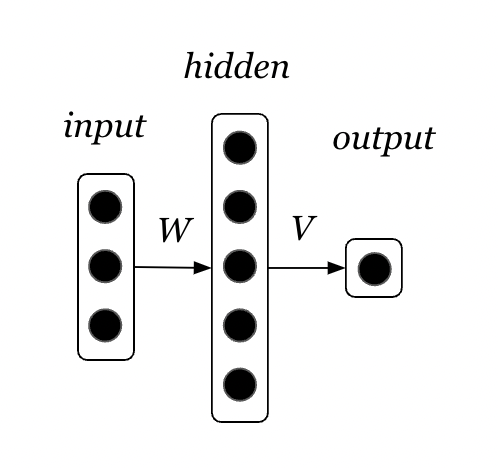
\includegraphics[width=0.3\textwidth]{images/fnn.png}
\caption{Example of a feedforward neural network}
\label{fig:fnn}
\end{figure}

\subsection{Recurrent Neural Network (RNN)}

\begin{figure}[ht]
\centering
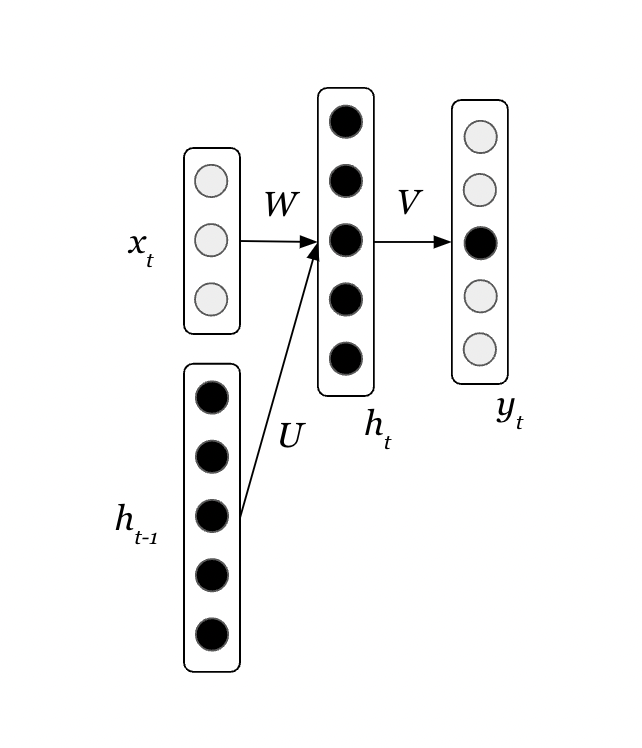
\includegraphics[width=0.4\textwidth]{images/rnn.png}
\caption{Example of a recurrent neural network (RNN)}
\label{fig:rnn}
\end{figure}

Recurrent neural networks are usually used to deal with sequences. They allow access to the input data as well as past data to compute the next state. As shown in Figure \ref{fig:rnn}, the hidden layer $h_t$ is computed using both input $x_t$ at time $t$ and the hidden state $h_{t-1}$ which contains the history information from time 0 to $t-1$. For each timestep $t$, the hidden state can be expressed as:
\[ h_t = Wx_t + Uh_{t-1} \]

\subsection{Recursive Neural Network (RvNN)}

\begin{figure}[ht]
\centering
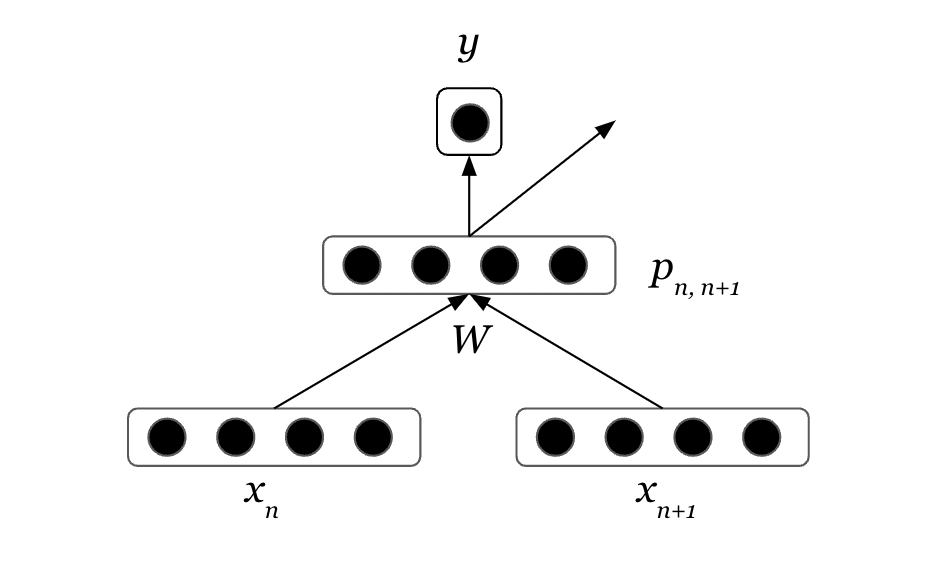
\includegraphics[width=0.6\textwidth]{images/rvnn.png}
\caption{Example of a recursive neural network (RvNN)}
\label{fig:rvnn}
\end{figure}

A recursive neural network has a tree-like structure. Figure \ref{fig:rvnn} illustrates an example of a basic RvNN architecture. The parent node representation is computed from its child nodes' representation as follows:
\[ p_{n, n+1} = f(W[x_n; x_{n+1}]) \]
where $f$ is the activation function. The same weight matrix $W$ will be applied recursively over the input.

\subsection{\texorpdfstring{Recursive Recurrent Neural Network (R\textsuperscript{2}NN)}{Recursive Recurrent Neural Network (R2NN)}}
The R\textsuperscript{2}NN proposed by Liu et al.\cite{r2nn} combines the features of RvNN and RNN. It has a tree-like structure similar to RvNN, with recurrent vectors added to integrate global information. As shown in Figure \ref{fig:r2nn}, $s^{[l, m]}$ and $s^{[m, n]}$ is the representation of child nodes $[l, m]$ and $[m, n]$. The recurrent input vectors, $x^{[l, m]}$ and $x^{[m, n]}$ are added to the two child nodes respectively. They encode the global information, such as language model scores and distortion model scores. A third recurrent input vector $x^{[l, n]}$ is added to the parent node $[l, n]$. The parent node representation is computed as
\[ s_j^{[l, n]} = f(\sum_{i} \hat{x}_i^{[l, n]}w_{ji}) \]
where $\hat{x}$ is the concatenation of vectors $[x^{[l, m]}; s^{[l, m]}; x^{[m, n]}; s^{[m, n]}]$, and $f$ is the $HTanh$ function. The output, $y^{[l, n]}$, is computed as
\[ y^{[l, n]} = \sum_{j} ([s^{[l, n]}; x^{[l, n]}])_{j}v_j \]


\begin{figure}[ht]
\centering
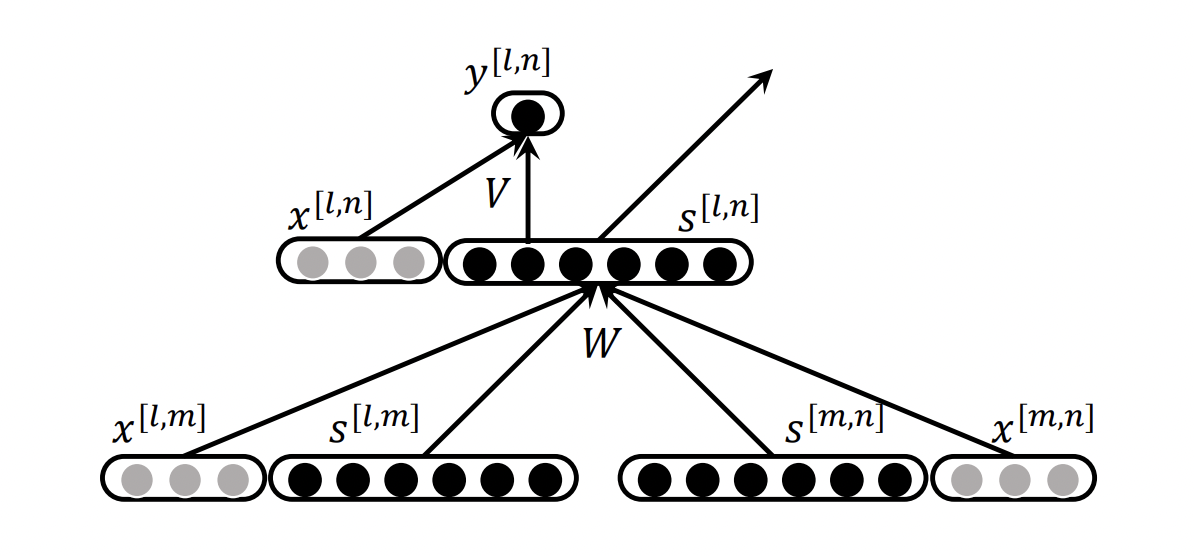
\includegraphics[width=0.6\textwidth]{images/r2nn.png}
\caption{Recursive recurrent neural network (Liu et al., 2014, p.1494)}
\label{fig:r2nn}
\end{figure}


\section{Requirement Analysis}

Based on the Project Structure section from my project proposal, the following requirements have been identified:

\textbf{Data preprocessing}
\begin{itemize}
    \item Data should be prepared in a form that is accepted by Moses SMT and R\textsuperscript{2}NN SMT
    \item Preprocessing should be done carefully to avoid accidentally correcting some of the grammatical errors 
    
    \begin{itemize}
        \item E.g. capitalisation errors may go undetected if all sentences are lowercased during data preprocessing
    \end{itemize}
\end{itemize}

\textbf{Moses SMT for GEC}
\begin{itemize}
    \item A language model should be trained to model the probability of a given sentence being valid
    \item A translation model should be trained to construct a phrase translation table
    \item A reordering model should be trained to learn the reordering of phrases
    \item With the above three models and Moses decoder, a complete Moses SMT system should be built
\end{itemize}

\textbf{R\textsuperscript{2}NN SMT for GEC}

Following the R\textsuperscript{2}NN paper by Liu et al.\cite{r2nn},
\begin{itemize}
    \item Phrase pair embeddings (PPE) should be learned by building a one-hidden-layer neural network and a recurrent neural network
    \item A recursive recurrent neural network (R\textsuperscript{2}NN) should be built and used as a decoder
\end{itemize}

\textbf{Evaluation}
\begin{itemize}
    \item The performance of both SMT systems should be evaluated using F0.5 scores
\end{itemize}

\section{Choice of Tools}

\subsection{Programming Language}

Python is chosen to be the main programming language as it provides many libraries that are commonly used for natural language processing. For this project I will be using \texttt{python 3.8} and PyCharm as my IDE.

\subsection{Libraries}
\textbf{PyTorch} \\
The \texttt{PyTorch}\footnote{https://pytorch.org/} library is one of the most popular machine learning frameworks. There are other similar libraries (such as \texttt{TensorFlow}) but I find \texttt{PyTorch} tutorials are easier to follow.

\textbf{NumPy} \\
My project is likely to involve statistical processing. I would be using the \texttt{NumPy}\footnote{https://numpy.org/} library for this purpose.

\textbf{pandas} \\
\texttt{pandas}\footnote{https://pandas.pydata.org/} is a powerful library for processing tabular data. This would be used to manipulate phrase tables in my project.

\subsection{Dataset}
The dataset introduced in BEA 2019 Shared Task\cite{bryant-etal-2019-bea} will be used in this project. I chose the corpora (\textbf{FCE v2.1}) which is immediately downloadable from the website\footnote{https://www.cl.cam.ac.uk/research/nl/bea2019st/\#data} to start with. The corpora have been standardised to be easily evaluated by ERRANT\cite{bryant-etal-2017-automatic}\cite{felice-etal-2016-automatic}. ERRANT is a toolkit used to annotate parallel data and compare hypothesis against reference to produce various evaluation metrics including F0.5 score. I may request other corpora as an extension of my project.

For language model training, I will be using the \textbf{One Billion Word} dataset\cite{one-billion-word}. This is a dataset used for language modeling and is available on GitHub\footnote{https://github.com/ciprian-chelba/1-billion-word-language-modeling-benchmark}.

\subsection{Version Control and Backup}
Git will be used for version control. The entire project, including all the written code and my dissertation, will be pushed to GitHub regularly.


\chapter{Implementation}
This chapter describes the implementation of a Moses baseline SMT system and an R\textsuperscript{2}NN SMT system. Since the main purpose of this project is to compare the performance of R\textsuperscript{2}NN decoder against Moses decoder, the R\textsuperscript{2}NN system should use the same language model, translation model and reordering model as Moses. For the translation model, the R\textsuperscript{2}NN paper\cite{r2nn} proposed a \textit{translation confidence based phrase pair embedding} (TCBPPE) to be used with the R\textsuperscript{2}NN decoder. The TCBPPE will base on a phrase table produced by Moses translation model. In the end, the R\textsuperscript{2}NN decoder will make use of language model scores, translation model scores, reordering model scores from Moses and TCBPPE to find the best translation candidate.

\begin{figure}[ht]
\centering
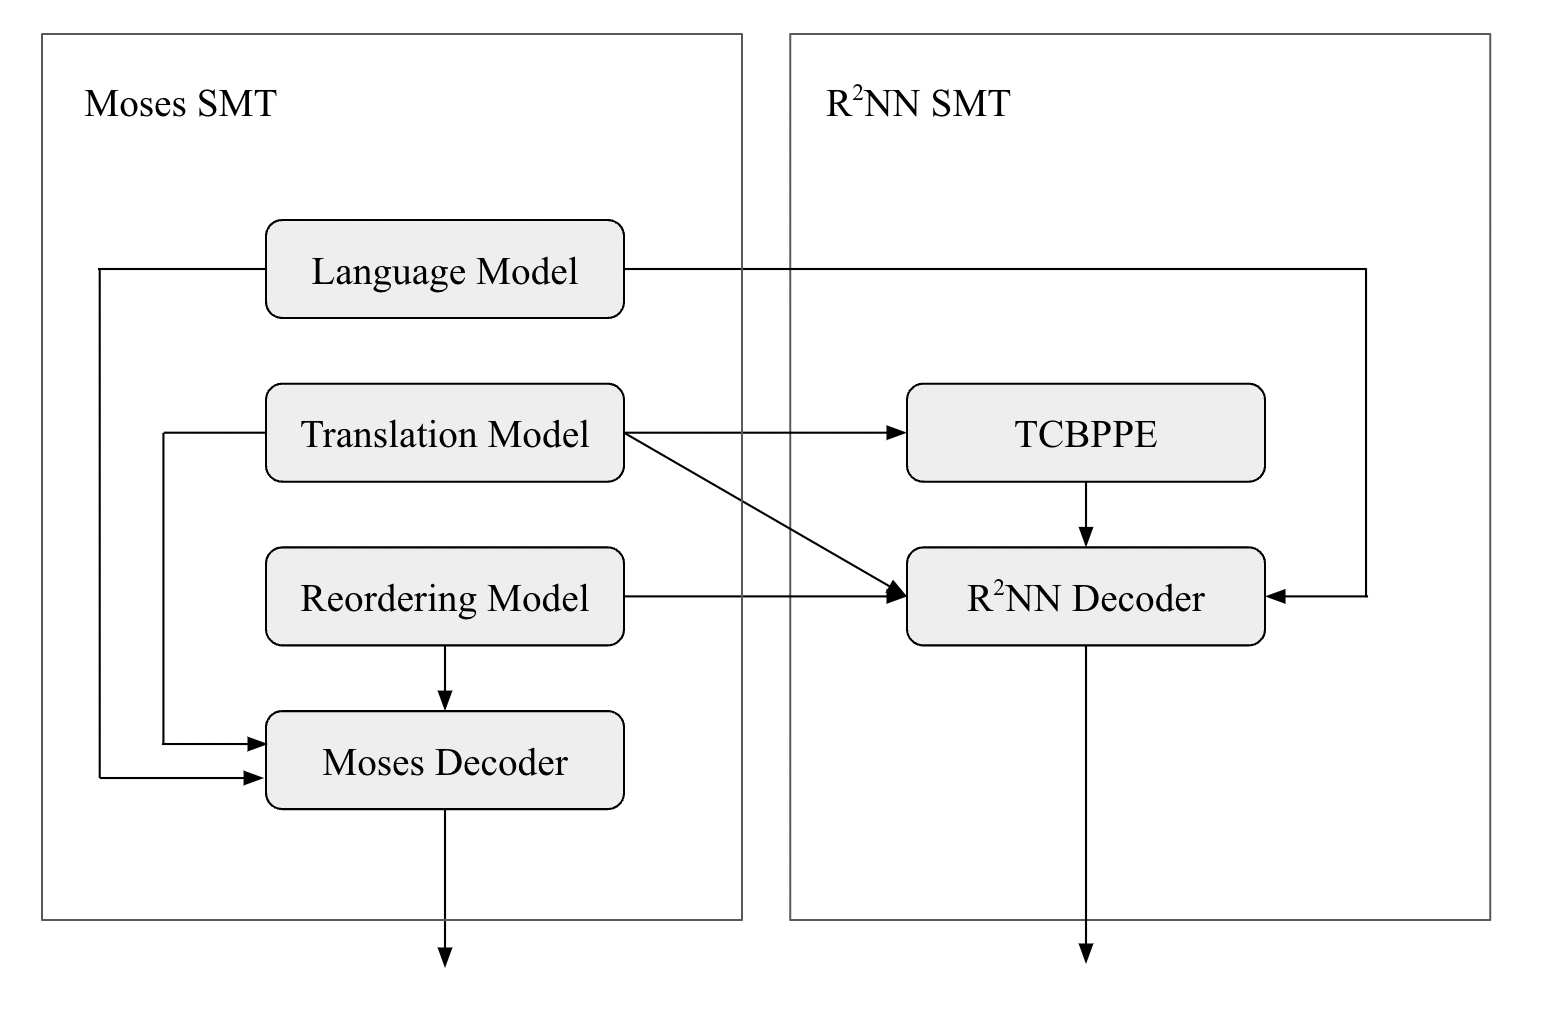
\includegraphics[width=0.9\textwidth]{images/overview_moses_r2nn.png}
\caption{Overview of Moses SMT and R\textsuperscript{2}NN SMT}
\label{fig:moses_r2nn}
\end{figure}

\section{Setup}\label{section:setup}

\subsubsection{FCE Dataset}

The FCE dataset was provided in m2 format. However, Moses requires parallel data which is aligned at the sentence level. An example taken from the m2 file looks like this:

\texttt{S} \textit{Her friend Pat had explained the whole story at her husband .}\\
\texttt{A 8 9|||R:PREP|||to|||REQUIRED|||-NONE-|||0}

[This means that for source sentence S, the word at position 8 to 9 (\textit{at}) should be corrected to \textit{to}.]

The m2 format needs to be converted to sentence-aligned data to be used by Moses. Two files are generated from this, where the source file contains\\
\textit{Her friend Pat had explained the whole story at her husband .}

and the target file contains\\
\textit{Her friend Pat had explained the whole story to her husband .}

\subsubsection{One Billion Word Dataset}

I downloaded the One Billion Word dataset for language model training. However, the files were too large to be handled by my machine. Since the dataset consists of fifty files, I decided to randomly choose 10 files from them and concatenated these files to be used in language model training. 


\section{Moses Baseline} \label{section:moses_baseline}

\begin{figure}[ht]
\centering
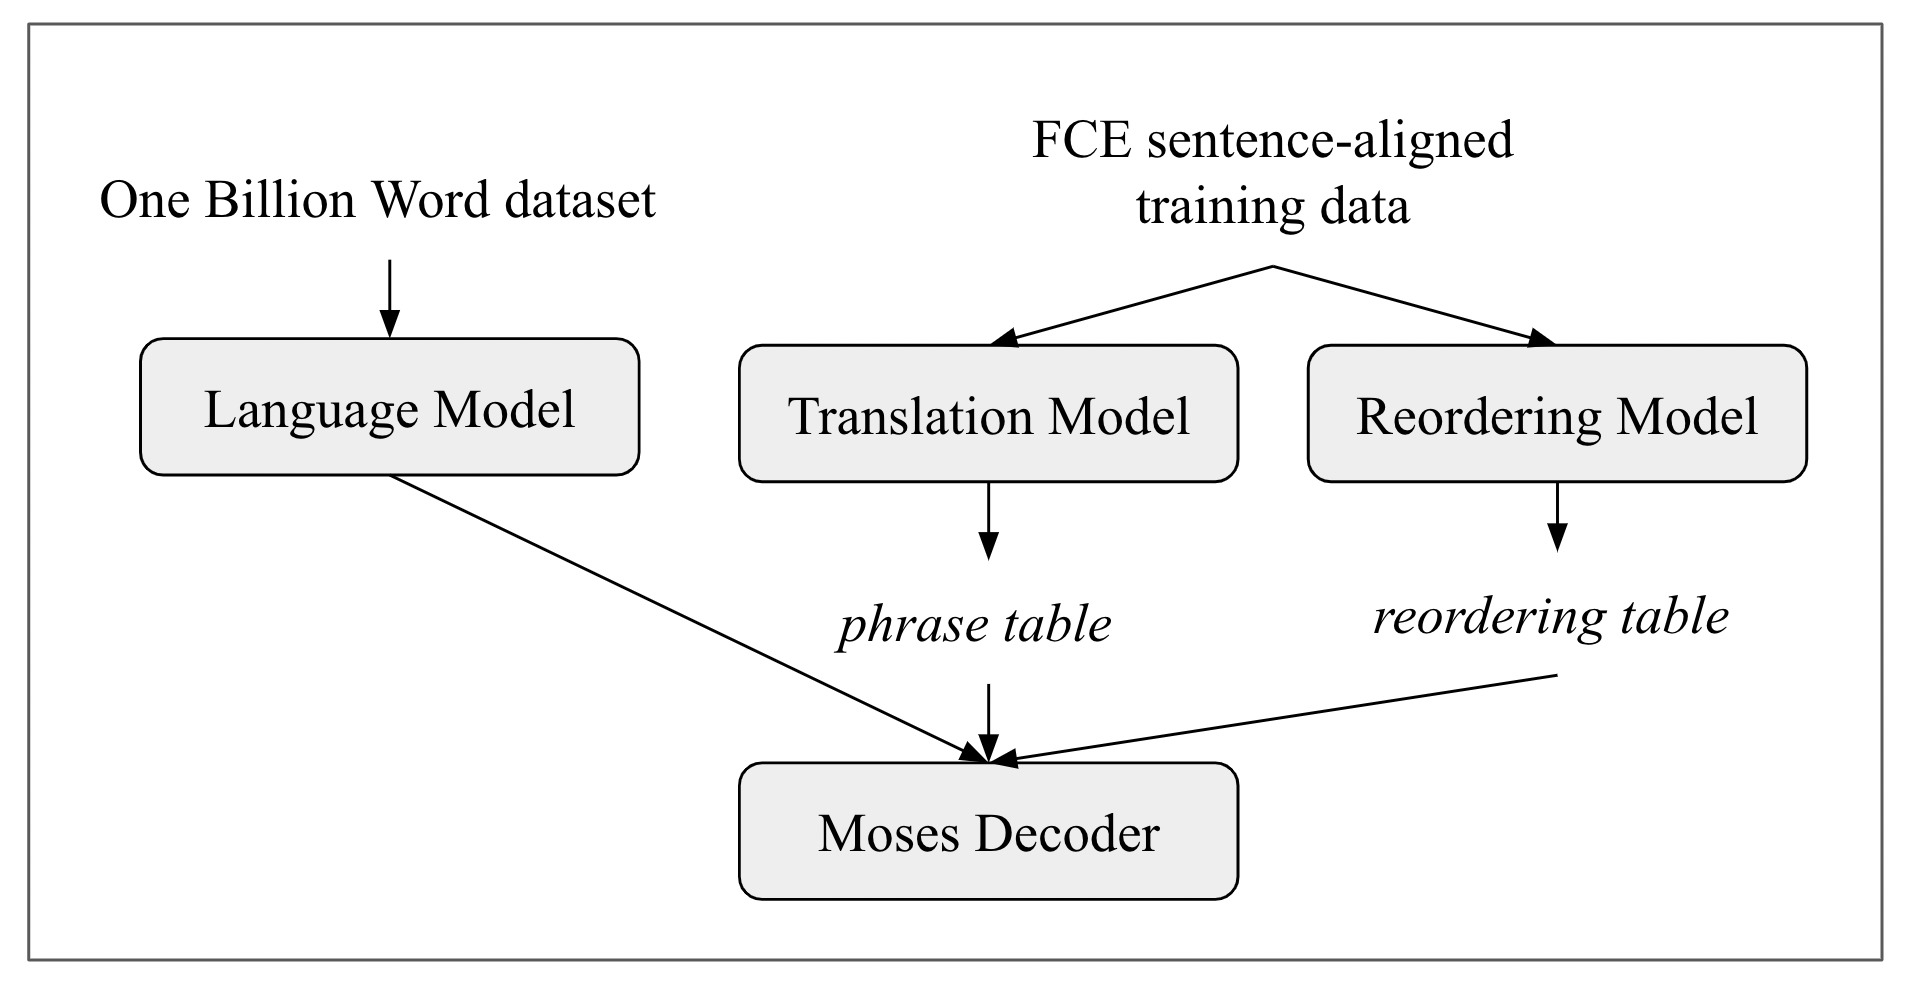
\includegraphics[width=0.8\textwidth]{images/moses_pipeline.png}
\caption{Overview of Moses SMT (training)}
\label{fig:moses_pipeline}
\end{figure}

\subsection{Language Model}
The One Billion Word dataset is used for language model training. In the R\textsuperscript{2}NN paper, a 5-gram language model is used. Here, I used KenLM which came with Moses installation to train a 5-gram language model. After training, the resulting language model is named \texttt{billion-training-monolingual-10.blm.en}. The following command is used to query the language model:
\begin{verbatim}
    ~/github/mosesdecoder/bin/query -n 
        /path/to/billion-training-monolingual-10.blm.en < queries.txt
\end{verbatim}

where \texttt{queries.txt} contains the sentences to be scored by the language model. For each sentence, the language model would return a total score (language model score), which is the log probability of this sentence. The example below shows that our trained language model assigns a higher score to a valid English sentence compared to incorrect English sentences.

\hfill\begin{minipage}{\dimexpr\textwidth-1cm}
    \textit{I have an apple .} LM score: $-9.682597$\\
    \textit{I have apple .} LM score: $-11.434978$\\
    \textit{I has apple .} LM score: $-13.841325$
\end{minipage}

\subsection{Translation Model and Reordering Model}
The translation model is trained with FCE sentence-aligned data. There are three components in translation model training: word alignment, phrase extraction and scoring. Word alignment is obtained using GIZA++, a toolkit to train word alignment models. Phrases are then extracted from our training files and a phrase table is produced. The phrase table contains phrase translation pairs and the scores associated with each pair. A distance-based reordering model is also built, and a reordering table is created. 

\begin{table}[ht]
\centering
\begin{tabular}{ |c|c|c|c|c| } 
 \hline
 source & target & scores & alignment & counts \\ [0.5ex] 
 \hline
 As we & As we & 1 0.901657 0.846154 0.90511 & 0-0 1-1 & 11 13 11\\
 As we & We & 0.00115075 1.68879e-05 0.0769231 0.0153198 & 1-0 & 869 13 1\\
 As we & as we & 0.0212766 0.00117032 0.0769231 0.00482726 & 0-0 1-1 & 47 13 1\\
 \hline
\end{tabular}
\caption{Phrase table from Moses}
\label{table:phrase_table}
\end{table}

After training, a configuration file named \texttt{moses.ini} is generated. By modifying the configuration file, we can change the language model, translation model and reordering model used by Moses decoder.

\section{\texorpdfstring{R\textsuperscript{2}NN}{R2NN} SMT}

\begin{figure}[ht]
\centering
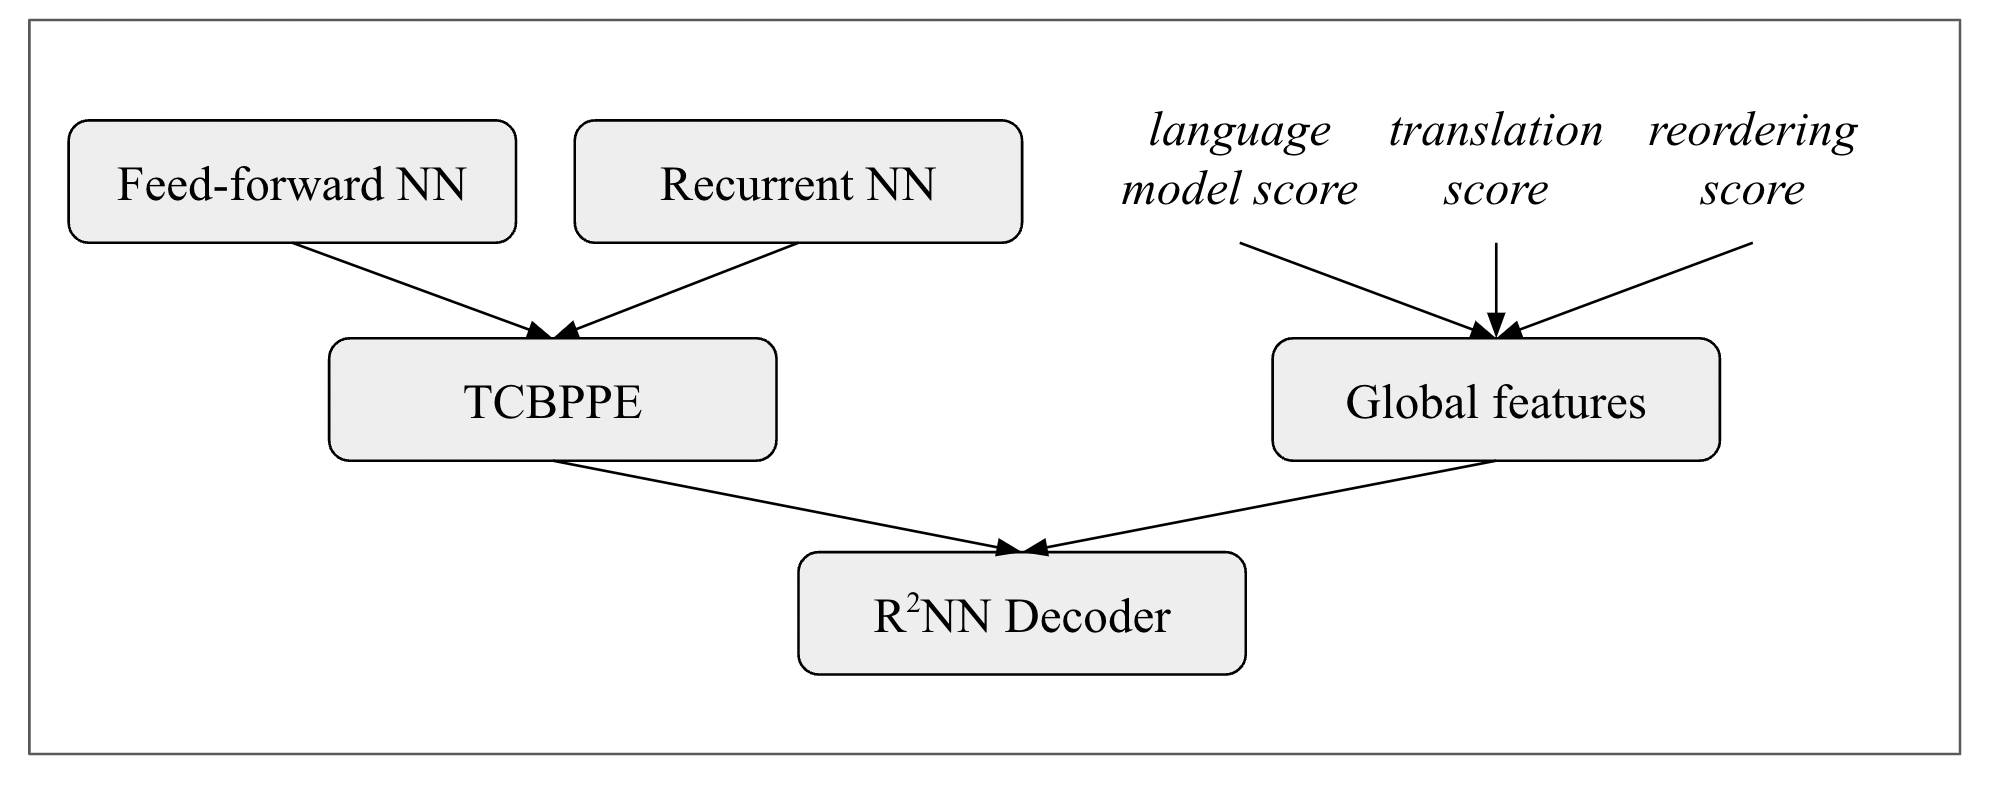
\includegraphics[width=1\textwidth]{images/r2nn_pipeline.png}
\caption{Overview of R\textsuperscript{2}NN SMT (training)}
\label{fig:r2nn_pipeline}
\end{figure}

The R\textsuperscript{2}NN SMT consists of three parts: translation confidence based phrase pair embedding (TCBPPE), global features, and an R\textsuperscript{2}NN decoder.

\subsubsection{TCBPPE}
A phrase pair embedding is a vector representation which encodes the meaning of a phrase pair. Recall that R\textsuperscript{2}NN model has a tree structure, where each node has a representation vector $s$ and a recurrent vector $x$. The TCBPPE is to be used as the representation vector $s$ and it is used to generate the leaf nodes of the derivation tree. 

The phrase pair embedding is split into two parts: translation confidence with sparse features and translation confidence with recurrent neural network. These two vectors will be obtained separately, and will be concatenated to be used as the representation vector $s$ in the R\textsuperscript{2}NN.

\subsubsection{Global features}
The global features encode global information that cannot be generated by child representations. It includes language model scores, translation scores and reordering scores which are obtained from Moses. These scores are concatenated together to be used as recurrent vectors $x$ to the R\textsuperscript{2}NN model.

\subsubsection{R\textsuperscript{2}NN decoder}
The recursive recurrent neural network (R\textsuperscript{2}NN) will be used as a decoder to find the best translation candidate. For an input sentence, the decoder would construct a tree based on phrases in the sentence. An output score will be computed based on TCBPPE, global features and the structure of the tree. The translation candidate that gives the highest score will be taken as the best translation candidate.

\subsection{TCBPPE: Sparse Features} \label{section:TCBPPE_sparse}

\begin{figure}[ht]
\centering
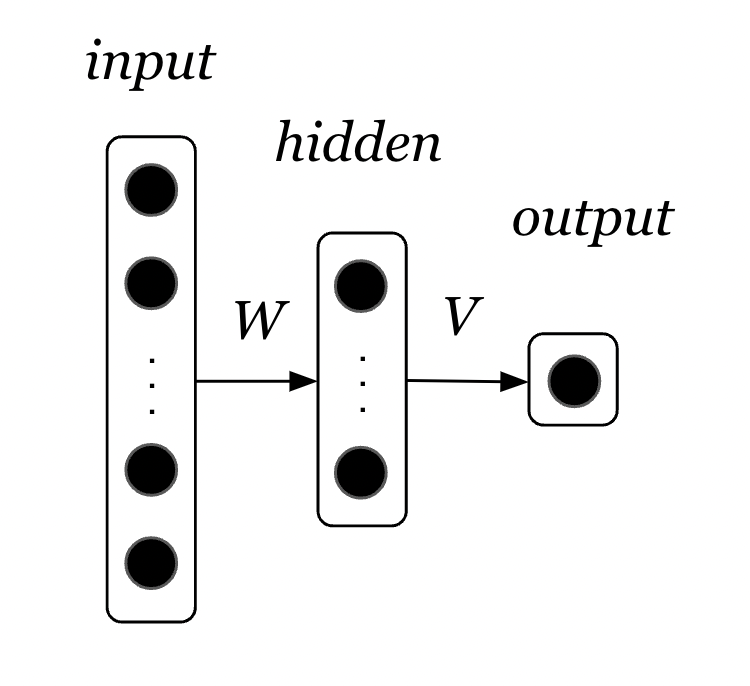
\includegraphics[width=0.3\textwidth]{images/one_hidden_layer.png}
\caption{Structure of one-hidden-layer feedforward neural network}
\label{fig:one_hidden_layer}
\end{figure}

A one-hidden-layer feedforward neural network is used to get a translation confidence score using sparse features. The structure of the network is shown in Figure \ref{fig:one_hidden_layer}. Following the R\textsuperscript{2}NN paper\cite{r2nn}, the size of the hidden layer is set to 20. The size of the input layer is 200,001. By training the network, we obtain hidden matrix $W$ of size 200,001 by 20. $W$ will be used as phrase pair embedding matrix for sparse features (\texttt{ppe\_sparse}). The goal is to find the $W$ that gives the best phrase pair embedding.

\subsubsection{Top phrase table}
A top phrase table \texttt{pt\_top} will be used when encoding training data. It contains the top 200,000 most frequent phrase pairs that appeared in the training data. We can obtain \texttt{pt\_top} from Moses phrase table using \texttt{pandas}. Recall that a column named "counts" is given in Moses phrase table (Table \ref{table:phrase_table}). It contains three numbers: the first is the number of times the target phrase appeared in training target file; the second is the number of times the source phrase appeared in training source file; the third is the number of times that the source phrase is mapped to the target phrase. To find the 200,000 most frequent phrase pairs, we can use \texttt{pandas} to perform a sort on "counts", and keep the top 200,000 rows. If \texttt{pt} is the phrase table loaded by \texttt{pandas}, then

\begin{verbatim}
    pt[["count_co", "count_or", "count_or_co"]] 
                            = pt["count"].str.split(expand=True)
    pt_sort = pt.sort_values(["count_or_co", "count_co", "count_or"], 
                            ascending=False)
    most_freq_pt = pt_sort.head(200000)
\end{verbatim}

would result in a table with 200,000 rows after sorting the counts column in descending order, with priority of
\[\textrm{phrase pair count} > \textrm{target count} > \textrm{source count}\]

\subsubsection{Prepare training data}
Next, we need to encode the training data (sentences) as one-hot like data to be used as input to the network. The phrase pairs in \texttt{pt\_top} will each be a feature, and an additional feature is used for all the infrequent phrase pairs. For each sentence pair (source-target) in the training data, it needs to be encoded as a vector of length 200,001 consisting of 0s and 1s, where the position $i$ in the vector contains a 1 if and only if the $i$\textsuperscript{th} most frequent phrase pair is found in this sentence pair. An example taken from the training file is shown below.

\textbf{Source sentence}
\textit{What she would do ?}

\textbf{Target sentence}
\textit{What would she do ?}

\textbf{Encoded vector}
\texttt{[$\underset{0}{0}, \ldots, \underset{39}{1}, \ldots, \underset{200000}{1}$]}

A 0 at position 0 means that the most frequent phrase pair does not exist in the sentence pair. A 1 at position 39 means that the 40\textsuperscript{th} most frequent phrase pair exists in the sentence pair. A 1 at position 200,000 means that the sentence pair contains a phrase pair that is not in the top 200,000 most frequent pairs.

\begin{table}[ht]
\centering
\begin{tabular}{ |c|c|c|c| } 
 \hline
 index & source & target & \ldots \\ [0.5ex] 
 \hline
 0 & . & . & \ldots \\ 
 \ldots & \ldots & \ldots & \ldots \\ 
 39 & do & do & \ldots \\ 
 \hline
\end{tabular}
\caption{Top 200,000 phrase pairs}
\label{table:pt_top_exmaple}
\end{table}

One problem with this is that the resulting vector from sentence pairs are usually sparse vectors. To save memory, instead of storing the whole vector, the position indices of 1s in the vector are stored in a file named \texttt{phrase\_pair\_id} (i.e. the phrase pair ids used in each sentence pair are stored). When loading the sentence pairs as training data, it is easy to obtain the one-hot encoding of each sentence pair from \texttt{phrase\_pair\_id}.

The next step is to obtain the expected output for each input sentence pair. Since the TCBPPE encodes translation model information, it is reasonable to use the translation scores from Moses translation model. For each sentence pair $S\textrm{-}T$ containing phrase pairs $p_1, p_2, ..., p_n$, the expected output score is computed by
\[ score_{S\textrm{-}T} = \frac{\sum_n c_{p_n}}{n} \]
where $c_{p_n}$ is the average translation score for phrase pair $p_n$.

\begin{figure}[ht]
\centering
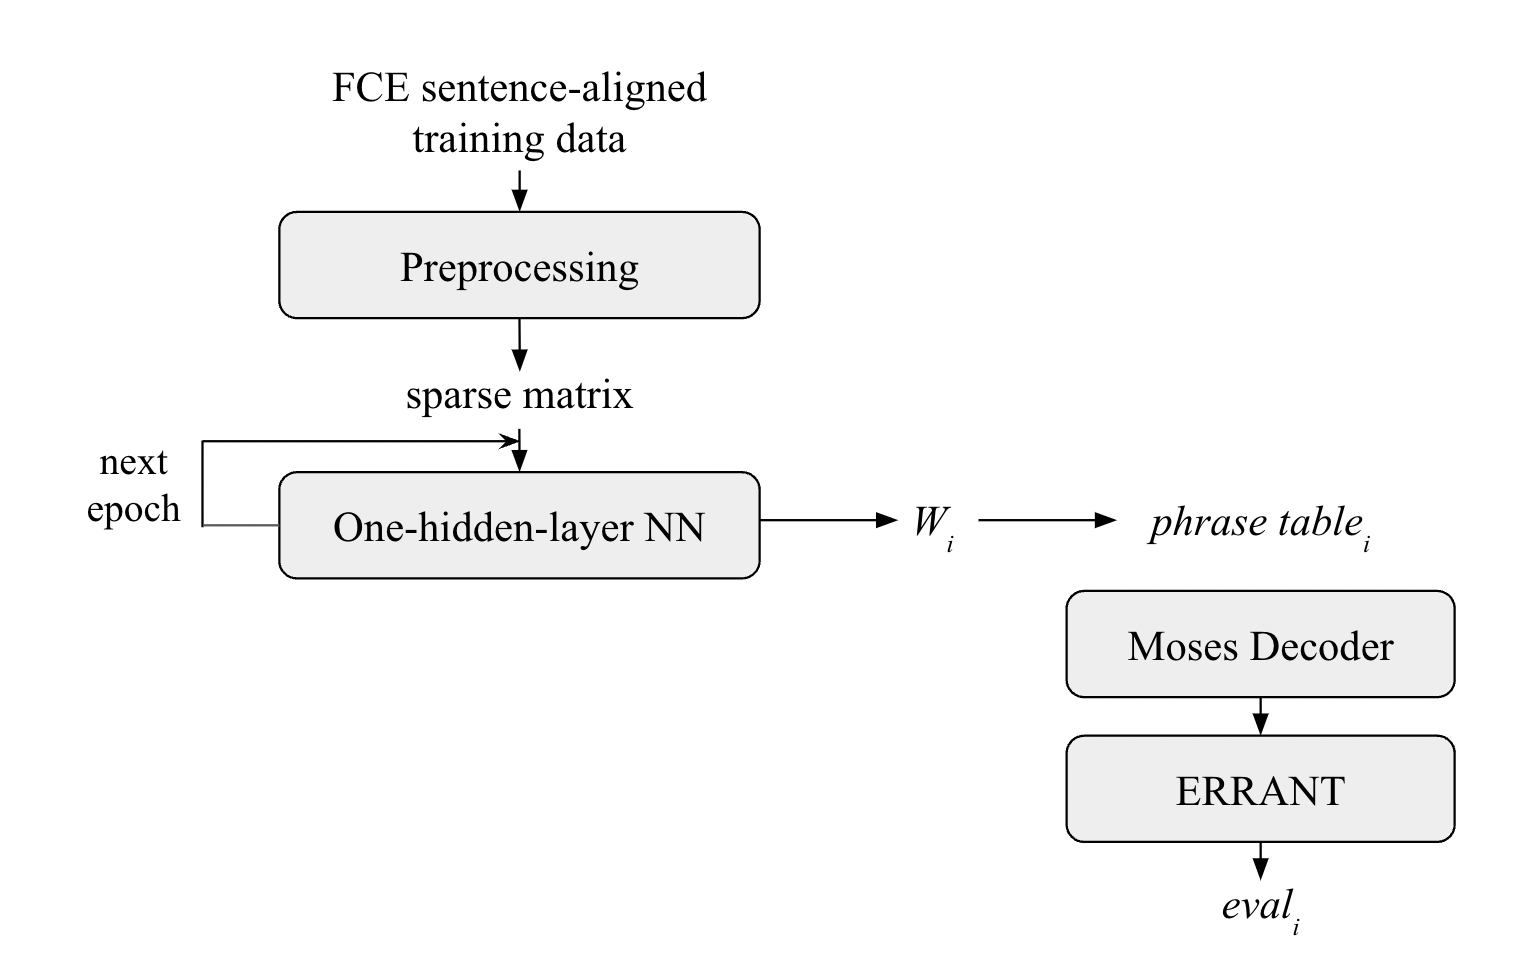
\includegraphics[width=0.8\textwidth]{images/sparse_pipeline.png}
\caption{Training pipeline of one-hidden-layer feedforward neural network}
\label{fig:sparse_pipeline}
\end{figure}

\subsubsection{Training one-hidden-layer neural network}

After obtaining the training dataset, we can train the neural network. The neural network will be trained for 10 epochs, where one epoch refers to one cycle of processing all the data in training set. After each epoch, the hidden matrix $W$ is stored. The $k^{th}$ row in $W$ will be used as the phrase pair embedding (sparse) for the top $k^{th}$ frequent phrase pair. That is, the embedding for the most frequent phrase pair is $W[0]$, and the embedding for phrase pairs that are not in the top 200,000 is represented by $W[200000]$.

We evaluate $W$ by updating Moses phrase table: for each row (ppe) in $W$, we add the ppe as an additional feature to the phrase table. Then we pass the updated phrase table to Moses decoder and use ERRANT to evaluate the performance. Table \ref{table:sparse_5} and Table \ref{table:sparse_10} shows the evaluation result by ERRANT for training epoch 5 and training epoch 10 respectively. Among all the $W$ from epoch 1 to 10, 10-epoch $W$ gives the highest precision, recall and $F_{0.5}$ score. Hence, $W$ will be used as the ppe matrix for sparse features (\texttt{ppe\_sparse}).

\begin{table}[ht]
    \centering
    \begin{tabular}{ |c|c|c|c|c|c| } 
     \hline
     TP & FP & FN & Prec & Rec & F0.5 \\ [0.5ex] 
     \hline
     543 & 2366 & 4006 & 0.1867 & 0.1194 & 0.1677 \\ 
     \hline
    \end{tabular}
    \caption{ERRANT output after training for 5 epochs}
    \label{table:sparse_5}
    
    \vspace{1em}
    
    \begin{tabular}{ |c|c|c|c|c|c| } 
     \hline
     TP & FP & FN & Prec & Rec & F0.5 \\ [0.5ex] 
     \hline
     545 & 2363 & 4004 & 0.1874 & 0.1198 & 0.1684 \\ 
     \hline
    \end{tabular}
    \caption{ERRANT output after training for 10 epochs}
    \label{table:sparse_10}
\end{table}

\subsection{TCBPPE: Recurrent Neural Network (RNN)} \label{section:TCBPPE_rnn}

\begin{figure}[ht]
\centering
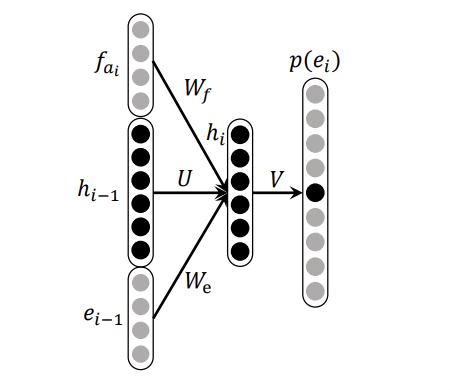
\includegraphics[width=0.4\textwidth]{images/rnn_ppe.png}
\caption{Recurrent neural network for translation confidence (Liu et al., 2014, p.1497)}
\label{fig:rnn_ppe}
\end{figure}

The other part of TCBPPE is generated by a recurrent neural network (RNN). The structure of the RNN used in shown in Figure \ref{fig:rnn_ppe}, where $e_i$ is the source word embedding, and $f_{a_i}$ is the word embedding of the target word which is aligned to $e_i$. The translation confidence score from source $s$ to target $t$ is given by
\[ T_{S2T}(s, t) = \sum_{i} \log p(e_i|e_{i-1}, f_{a_i}, h_i)\]

\subsubsection{Building RNN}
Firstly, we need to decide what to use for word embeddings. There are several popular pre-trained word embeddings available, such as GloVe\footnote{https://nlp.stanford.edu/projects/glove/} and fastText\footnote{https://fasttext.cc/docs/en/crawl-vectors.html}. I have chosen fastText pre-trained models because fastText is based on character n-grams, whereas GloVe takes a word to be the smallest unit. For the task of Grammatical Error Correction, it is likely that OOV (out of vocabulary) words will occur in the source (such as misspelled words). fastText can easily generate word embeddings for those unseen words based on character n-grams.

Next step is to construct a PyTorch dataset from the FCE training data. For each $S\textrm{-}T$ sentence pair, we obtain $e_i$ and $e_{i-1}$ from source $S$ and $f_{a_i}$ from target $T$. Then we define a class for RNN as follows:

\begin{verbatim}
    class RecurrentNN(torch.nn.Module):
        def __init__(self, input_size, hidden_size, output_size):
            super(RecurrentNN, self).__init__()
            self.U = torch.nn.Linear(input_size+hidden_size, hidden_size)
            self.V = torch.nn.Linear(hidden_size, output_size)
            self.softmax = torch.nn.LogSoftmax(dim=1)
\end{verbatim}

where \texttt{input\_size} should be size of word embedding multiplied by 2 (since it is $e_{i-1}$ and $f_{a_i}$ concatenated together). The size of word embedding is set to 50 to avoid memory issues, and the size of hidden layer is set to 100. The \texttt{torch.nn.LogSoftmax} layer would convert output to a categorical probability distribution, hence the \texttt{output\_size} should be the size of vocabulary in our training data.

\subsubsection{Training RNN}
We train the RNN for 3 epochs and store the model state. Then, we load the model and run the model on the top phrase table \texttt{pt\_top}. For each phrase pair from source phrase $s$ to target phrase $t$, we compute 
\[ T_{S2T}(s, t) = \sum_{i} \log p(e_i|e_{i-1}, f_{a_i}, h_i)\]
and save $T_{S2T}(s, t)$ to be the phrase pair embedding with RNN (\texttt{ppe\_rnn}). 

\subsection{Global Features} \label{section:global_features}
Three features are proposed to be used as global features, namely language model score, translation model score and reordering model score. Language model scores can be obtained by querying the trained 5-gram KenLM language model. Translation model scores are accessible from Moses phrase table. However, although a reordering table was created by Moses after training, it is unclear what each score means and Moses documentation did not give details of the reordering score components. Hence, the reordering scores are omitted and only translation model score and language model score will be used as global features in R\textsuperscript{2}NN decoder.

\subsubsection{Translation model scores}
The translation model scores are calculated by taking the average of the four scores given by each phrase pair in the phrase table. If \texttt{pt} is the phrase table loaded by \texttt{pandas}, we could calculate the translation model score for each phrase pair by

\begin{verbatim}
    pt["confidence"] = pt["scores"].map(
                        lambda scores: round(
                        sum([float(i) for i in scores.split()])/4, 6))
\end{verbatim}

The result will be stored in a file named \texttt{pt\_top\_id\_confidence}.

\subsubsection{Language model scores}
We obtain the language model scores for the target phrase by querying the language model:
\begin{verbatim}
    ~/github/mosesdecoder/bin/query 
        -n /path/to/billion-training-monolingual-10.blm.en 
        < pt_top_target
        > lm_total_scores
\end{verbatim}

where \texttt{billion-training-monolingual-10.blm.en} is the binarised trained language model, \texttt{pt\_top\_target} is the file containing target phrases, one per line, and the output of this command is saved in \texttt{lm\_total\_scores}. We can write the language model score to the phrase table and name it \texttt{pt\_top\_lm}.


\subsection{\texorpdfstring{R\textsuperscript{2}NN}{R2NN} Decoder} \label{section:r2nn_model}
Recall that in Figure \ref{fig:r2nn}, each node in R\textsuperscript{2}NN consists of two parts: $s$ for the representation of the phrase (TCBPPE), and $x$ for the recurrent input vectors (global features). Let's first define two functions, \texttt{get\_ppe} and \texttt{get\_rec} which would return $s$ and $x$ respectively for any given source phrase and target phrase.

\subsubsection{Obtain representation vector (TCBPPE)}
We obtained two files, \texttt{ppe\_sparse} and \texttt{ppe\_rnn}, from section \ref{section:TCBPPE_sparse} and \ref{section:TCBPPE_rnn}. We combine them to be the TCBPPE (\texttt{ppe\_matrix}):

\begin{verbatim}
    ppe_matrix = np.zeros((200001, 21))
    ppe_matrix[:, 0:20] = ppe_sparse
    ppe_matrix[0:200000, 20] = ppe_rnn
\end{verbatim}

and the phrase pair embedding for the top $i^{th}$ phrase pair is accessed by \texttt{ppe\_matrix[i]} and is of length 21. \texttt{ppe\_matrix[200000]} is used for any phrase pair that is not in the top 200,000 frequent ones. We can define \texttt{get\_ppe} as

\begin{verbatim}
    def get_ppe(source_phrase, target_phrase):
        mappings = pt_top_lm.loc[(pt_top_lm["source"] == source_phrase) 
                                & (pt_top_lm["target"] == target_phrase)]
        ...
\end{verbatim}

and return \texttt{ppe\_matrix[200000]} if \texttt{mappings} is empty (i.e. no such phrase pair found in the top phrase table), otherwise return \texttt{ppe\_matrix[mapping\_id]}.

\subsubsection{Obtain recurrent vector (Global features)}
The recurrent vector consists of two scores: the translation model score and the language model score. From section \ref{section:global_features}, we created \texttt{pt\_top\_id\_confidence} for translation model scores, and \texttt{pt\_top\_lm} for language model scores. With the help of these files, we can define \texttt{get\_rec}. Similar to \texttt{get\_ppe}, we first obain mappings from source phrase to target phrase. Then we look up the scores in \texttt{pt\_top\_id\_confidence} and \texttt{pt\_top\_lm} using \texttt{mapping\_id}.

\begin{verbatim}
    def get_rec(source_phrase, target_phrase):
        mappings = pt_top_lm.loc[(pt_top_lm["source"] == source_phrase) 
                                & (pt_top_lm["target"] == target_phrase)]
        ...
        t_score = pt_id_confidence.iloc[mapping_id]["confidence"]
        l_score = pt_top_lm.iloc[mapping_id]["lm"]
        return torch.tensor([t_score, l_score], dtype=torch.float32)
\end{verbatim}

If \texttt{mappings} is empty, both \texttt{t\_score} and \texttt{l\_score} will default to 0.

\subsubsection{Building recursive neural network (RvNN)}
There has not been any published implementation of R\textsuperscript{2}NN. However, since R\textsuperscript{2}NN has a tree-like structure, it is sensible to start with building a recursive neural network. A good example is given in a blog post\cite{rvnn_daniel}, where the recursive neural network is constructed from two parts: a class \texttt{TreeNode} which builds a greedy tree from the input, and a class \texttt{NeuralGrammar} which is the neural network that processes the tree. Following the post, I built a recursive neural network (RvNN) with similar structure:

\begin{verbatim}
    class RecursiveNN(torch.nn.Module):
        def __init__(self, input_size):
            super(RecursiveNN, self).__init__()
            self.W = torch.nn.Linear(input_size * 2, input_size)
            self.V = torch.nn.Linear(input_size, 1)
    
        def forward(self, node):
            ...
    
    class TreeNode:
        def __init__(self, representation=None):
            self.representation = representation
            self.left = None
            self.right = None
    
        def greedy_tree(self, x, model):
            ...
\end{verbatim}

The \texttt{greedy\_tree} function in class \texttt{TreeNode} takes argument \texttt{x} which is a list of representation of leaf nodes. It converts each leaf node representation to a \texttt{TreeNode} first, and then combine them in a greedy way. Based on the output of \texttt{model(combined\_tree)}, it chooses the combination of the nodes that gives the highest score.

To use \texttt{RecursiveNN}, we construct a tree from representation of leaf nodes $x$ and pass the tree to the neural network:

\begin{verbatim}
    rvnn = RecursiveNN(4)
    x = numpy.array([[8,8,8,8], [2,2,2,2], [3,3,3,3], [7,7,7,7]])
    tree_node = TreeNode()
    tree = tree_node.greedy_tree(x, rvnn)
    parent_node, score = rvnn(tree)
\end{verbatim}


\subsubsection{Building \texorpdfstring{R\textsuperscript{2}NN}{R2NN}}
To build R\textsuperscript{2}NN, we need to add recurrent input vector to the RvNN. Firstly, \texttt{ppe\_size} and \texttt{rec\_size} should be included in the initialisation signature. The size of $W$ should be (\texttt{ppe\_size} $+$ \texttt{rec\_size}) by \texttt{ppe\_size}, since the phrase pair embedding for parent node is generated from child nodes, whereas the recurrent input vector for parent node is independent of child nodes. The size of $V$ is (\texttt{ppe\_size} $+$ \texttt{rec\_size}) by 1 because output score is of size 1 and is generated from concatenation of phrase pair embedding and recurrent vector of parent node.

\begin{verbatim}
    class R2NN(torch.nn.Module):
        def __init__(self, ppe_size, rec_size):
            super(R2NN, self).__init__()
            self.input_size = ppe_size + rec_size
            self.W = torch.nn.Linear(self.input_size*2, ppe_size)
            self.V = torch.nn.Linear(self.input_size, 1)
\end{verbatim}

The \texttt{forward} function should use the \texttt{get\_rec} function defined in section \ref{section:r2nn_model} to obtain the recurrent input vector for parent node.

\begin{verbatim}
    def forward(self, node):
        ...
        parent_ppe = torch.tanh(self.W(inp_vector))
        parent_rec = get_rec(parent_source, parent_target)
        ...
\end{verbatim}

At the same time, when \texttt{greedy\_tree} function generate leaf tree nodes, it will make use of both \texttt{get\_ppe} and \texttt{get\_rec} to get tree node vector representation.

\subsubsection{Preprocessing training data}
Following the R\textsuperscript{2}NN paper\cite{r2nn}, forced decoding will be used to generate positive samples. We can perform forced decoding with Moses by adding the following line to Moses configuration file, \texttt{moses.ini}:
\begin{verbatim}
    ConstrainedDecoding path=/path/to/gold/standard/file
\end{verbatim}
where the gold standard file should be target sentences in FCE training dataset. Then we can pass the updated configuration file to Moses decoder and do forced decoding on source sentences in FCE training set. The phrase pairs used in forced decoding for each sentence is stored in a file named \texttt{phrases\_train}.

We define a function \texttt{process\_phrases\_file} to remove the sentences which did not give a forced decoding result in \texttt{phrases\_train}. For each of the remaining sentences, we extract phrase pairs used and a total score given by Moses decoder. Then we can construct a PyTorch dataset where the input is a list of phrase pairs used in each sentence and the expected output is the total score of that sentence.

\subsubsection{Training \texorpdfstring{R\textsuperscript{2}NN}{R2NN}}
We recall the loss function defined in R\textsuperscript{2}NN paper\cite{r2nn}
\[Loss(W,V,s^{[l,n]}) = \max{(0, 1-y_{oracle}^{[l,n]} + y_t^{[l,n]})} \]
where $y_{oracle}^{[l,n]}$ is the score from forced decoding (the expected score), and $y_t^{[l,n]}$ is the output score from R\textsuperscript{2}NN for a source span $s^{[l,n]}$. The $\max$ function is used to guarantee non-negative loss. Then we save the state of our trained model in \texttt{model\_state\_r2nn.pth}.

\section{Repository Overview}
\begin{figure}[ht]
    \begin{verbatim}
    errant/
    fastText/
    giza-pp/
    mosesdecoder/
    part-ii-project/
    ├── corpus/
    ├── evaluation/
    ├── helper_scripts/
    ├── lm/
    ├── model/
    │   ├── R2NN/
    │   │   ├── R2NN.py
    │   │   ├── get_ppe.py
    │   │   ├── obtain_pt_target.py
    │   │   ├── recursive_nn.py
    │   │   ├── save_top_lm.py
    │   │   ├── test_r2nn.py
    │   │   ├── train_r2nn.py
    │   │   └── r2nn_state/
    │   ├── RNN/
    │   │   ├── cc.en.50.bin
    │   │   ├── recurrent_nn.py
    │   │   ├── save_ppe_rnn.py
    │   │   ├── train_rnn.py
    │   │   └── rnn_state/
    │   ├── sparse/
    │   │   ├── calc_avg_feature.py
    │   │   ├── one_hidden_layer_net.py
    │   │   ├── one_hot_encode.py
    │   │   ├── save_ppe_sparse.py
    │   │   ├── top_phrase_table.py
    │   │   ├── train_one_hidden_layer.py
    │   │   ├── update_phrase_table.py
    │   │   ├── one_hidden_layer/
    │   │   └── phrase_tables/
    │   └── ...
    ├── moses_exp/
    │   ├── tuned_moses.ini
    │   └── ...
    └── project-reports/
    \end{verbatim}
    \caption{Repository Overview}
    \label{fig:repo}
\end{figure}

Figure \ref{fig:repo} shows the repository structure of my project. 

\texttt{errant/} contains a fork of the GitHub\footnote{https://github.com/chrisjbryant/errant} repository \texttt{chrisjbryant/errant}\cite{bryant-etal-2017-automatic}\cite{felice-etal-2016-automatic} which is used to annotate and score the hypothesis file (translated sentences) to the reference file (target sentences). 

\texttt{fastText/} contains a fork of the GitHub\footnote{https://github.com/facebookresearch/fastText} repository \texttt{facebookresearch/fastText}\cite{grave2018learning} which generates word embeddings in RNN training. The binarised model is saved to \texttt{part-ii-project/model/RNN/cc.en.50.bin}.

\texttt{giza-pp/} contains a fork of the GitHub\footnote{https://github.com/moses-smt/giza-pp} repository \texttt{moses-smt/giza-pp}\cite{giza_pp} and it is used in Moses SMT to obtain alignment models.

\texttt{mosesdecoder/} contains a fork of the GitHub\footnote{https://github.com/moses-smt/mosesdecoder} repository \texttt{moses-smt/mosesdecoder}\cite{moses}. Moses decoder, as well as tools for building associated models can be found here.

\texttt{part-ii-project/} is where the main code of the project resides. It contains:

\hfill\begin{minipage}{\dimexpr\textwidth-1cm}
    \texttt{corpus/} contains the downloaded FCE corpus as well as the preprocessed sentence-aligned FCE corpus.
\end{minipage}

\hfill\begin{minipage}{\dimexpr\textwidth-1cm}
    \texttt{evaluation/} contains the intermediate files and output files from ERRANT.
\end{minipage}

\hfill\begin{minipage}{\dimexpr\textwidth-1cm}
    \texttt{helper\_scripts/} contains scripts to preprocess FCE corpus and scripts to perform some simple tasks such as concatenating files.
\end{minipage}

\hfill\begin{minipage}{\dimexpr\textwidth-1cm}
    \texttt{lm/} contains the binary file of the language model from Moses.
\end{minipage}

\hfill\begin{minipage}{\dimexpr\textwidth-1cm}
    \texttt{moses\_exp/} is the working directory for Moses decoder and contains the intermediate files generated by Moses in section \ref{section:moses_baseline}.
\end{minipage}

\hfill\begin{minipage}{\dimexpr\textwidth-1cm}
    \texttt{model/} includes three sub-directories, \texttt{sparse/}, \texttt{RNN/} and \texttt{R2NN/}, as well as related files (such as the top phrase table \texttt{pt\_top}).
\end{minipage}

The following sections give further details of \texttt{part-ii-project/model/}.

\subsection{\texttt{sparse/}}
\texttt{top\_phrase\_table.py}\\
Process Moses phrase table to obtain the top 200,000 phrase pairs, \texttt{pt\_top}.

\texttt{one\_hot\_encode.py}\\
Encode sentences in FCE training dataset as one-hot like tensors.

\texttt{calc\_avg\_feature.py}\\
Calculate the expected feature score for each sentence in FCE training dataset.

\texttt{one\_hidden\_layer\_net.py}\\
Class definition for one-hidden-layer feedforward neural network.

\texttt{train\_one\_hidden\_layer.py}\\
Code to load the dataset and perform training.

\texttt{update\_phrase\_table.py}\\
Write the new features obtained from the neural network to the phrase table.

\texttt{save\_ppe\_sparse.py}\\
Save the parameter $W$ of the model to a file, \texttt{ppe\_sparse.npy}, to be the phrase pair embedding with sparse features.

\subsection{\texttt{RNN/}}
\texttt{recurrent\_nn.py}\\
Class definition for recurrent neural network (RNN).

\texttt{train\_rnn.py}\\
Code to load the dataset and perform training.

\texttt{save\_ppe\_rnn.py}\\
Save the output of RNN to a file, \texttt{ppe\_rnn.npy}, to be the phrase pair embedding with RNN.

\subsection{\texttt{R2NN/}}
\texttt{get\_ppe.py}\\
Combine \texttt{ppe\_sparse.npy} and \texttt{ppe\_rnn.npy} to be the phrase pair embedding matrix, \texttt{ppe\_matrix.npy}.

\texttt{obtain\_pt\_target.py}\\
Obtain all the target phrases from phrase table for querying Moses language model.

\texttt{save\_top\_lm.py}\\
Write the language model scores to the phrase table.

\texttt{R2NN.py}\\
Class definition for recursive recurrent neural network (R\textsuperscript{2}NN).

\texttt{train\_r2nn.py}\\
Code to process Moses forced decoding output, create a PyTorch dataset, and train the R\textsuperscript{2}NN.


\chapter{Evaluation}\label{chapter:evaluation}

\section{Success Criteria}\label{section:success_criteria}
All of the success criteria specified in the project proposal have been met and are presented below.
\begin{itemize}
    \item[\checkmark] Data is pre-processed for the use of training the models \textit{(section \ref{section:setup})}
    \item[\checkmark] A baseline SMT-based GEC system is built \textit{(section \ref{section:moses_baseline})}
    \item[\checkmark] A one-hidden-layer neural network is built to learn the translation confidence score \textit{(section \ref{section:TCBPPE_sparse})}
    \item[\checkmark] A recurrent neural network is built to learn the translation confidence score \textit{(section \ref{section:TCBPPE_rnn})}
    \item[\checkmark] An R2NN model is implemented \textit{(section \ref{section:global_features} and \ref{section:r2nn_model})}
    \item[\checkmark] An SMT-based GEC system making use of the R2NN decoder is built \textit{(section \ref{section:r2nn_model})}
    \item[\checkmark] A comparison between the performances of the two systems is performed \textit{(chapter \ref{chapter:evaluation})}
\end{itemize}

\section{Evaluation Metrics}
We use the same evaluation metrics as specified in the BEA 2019 Shared Task\cite{bryant-etal-2019-bea}, ERRANT scorer\cite{bryant-etal-2017-automatic}\cite{felice-etal-2016-automatic}, to evaluate the performance of Moses SMT-based GEC system and R\textsuperscript{2}NN SMT-based GEC system. Compared to other evaluation scripts commonly used in machine translation (such as BLEU\footnote{https://en.wikipedia.org/wiki/BLEU}), ERRANT is more informative for GEC because it computes $F_{0.5}$ score based on span-based correction.

The $F_{0.5}$ score is computed based on precision $P$ and recall $R$. Let $T_P$ be the true positive where system \textbf{correctly} made a change, $F_P$ be the false positive where the system \textbf{incorrectly} made a change, $F_N$ be the false negative where the system \textbf{missed} a change that it should have made. We can calculate precision
\[P = \frac{T_P}{T_P+F_P}\]
and recall
\[R = \frac{T_P}{T_P+F_N}\]

$F_{0.5}$ is the weighted harmonic mean of $P$ and $R$ and is computed as 
\[F_{0.5}=(1+0.5^2)\times\frac{P\times R}{0.5^2\times P+R}\]

\section{Testing}
We will use the held out FCE test set for testing. The m2 file of the FCE test set will be processed as described in section 3.1. We obtain two sentence-aligned files: one containing all the source sentences in the test set and one containing all the target sentences (gold reference). Moses decoder and R\textsuperscript{2}NN decoder will process the source file, and each system will produce a translation file which contains the translations of the source sentences. We can then use ERRANT to evaluate the translation file against the target file.

\subsection{Moses Decoder}
\begin{figure}[ht]
\centering
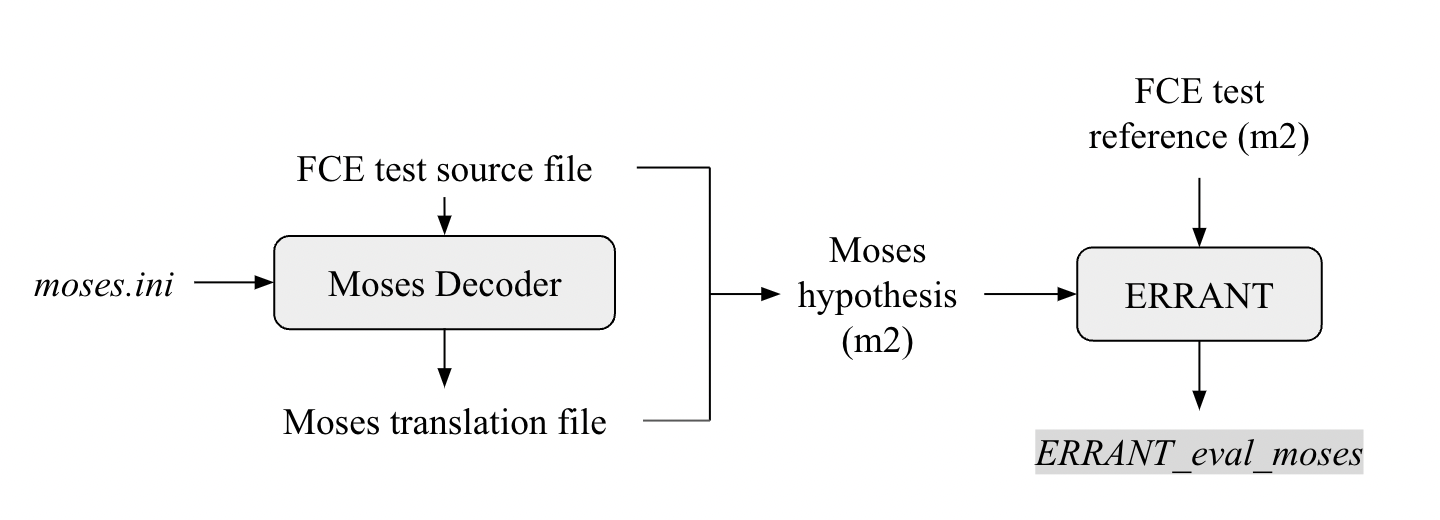
\includegraphics[width=0.9\textwidth]{images/moses_test.png}
\caption{Testing pipeline of Moses SMT}
\label{fig:moses_test}
\end{figure}

Before testing Moses decoder, we should tune the parameters using a small amount of parallel data which is different from the training data. We will use the FCE development set for this purpose. The tuning process would optimize the weights for each feature as specified in \texttt{moses.ini}. Then we can use Moses decoder to translate the test set:
\begin{verbatim}
    ~/github/mosesdecoder/bin/moses 
        -f /path/to/moses.ini 
        < /path/to/fce/test/source
        > fce.test.moses.translated
\end{verbatim}

where \texttt{fce.test.moses.translated} is the translation file produced by Moses decoder. We use ERRANT to annotate the source file with the translation file to obtain the hypothesis m2 file. After that, we can compute evaluation scores using ERRANT scorer and the result will be saved to \texttt{ERRANT\_eval\_moses}.

\subsection{\texorpdfstring{R\textsuperscript{2}NN}{R2NN} Decoder}\label{section:r2nn_test}
To use the R\textsuperscript{2}NN decoder, firstly we need to split the sentence into phrases. Liu et al. did not specify the method they used for phrase splitting in the paper\cite{r2nn}, so I came up with a greedy method: starting from the beginning word of a sentence, we look for the longest possible phrase that appears in our top phrase table. If a phrase is found, we keep the phrase and move on to the remaining part of the sentence; if no such phrases are found, we make that word a phrase, and move on to the next word. An example is given below.

\textbf{Sentence}\\
\textit{I hope that he will recover soon and that he will make it to our conference .}

\textbf{Sentence span}\\
\textit{I hope that /he will /recover /soon and /that he /will make /it to /our /conference /.}

The next step is to obtain phrase pairs based on the sentence span. For each phrase in the span, we have a list of possible phrase pairs. We use our R\textsuperscript{2}NN model to compute a score for each phrase pair and only keep the n-best phrase pairs. Then we recursively repeat the process and build a tree based on the phrase pairs. Every tree node has two attributes: \texttt{node.source} which gives the source phrase of this node and \texttt{node.target} which gives the target phrase. The translation for a sentence can be obtained by accessing the root node's \texttt{target} attribute of the tree. The resulting translation file will be saved to \texttt{ERRANT\_eval\_r2nn}.

\textbf{Phrase pairs}\\
\textit{(I hope that $\rightarrow$ I hope that),
        (I hope that $\rightarrow$ I hope),
        \dots}

However, when it comes to testing, I discover that the search space is too big for my laptop to process. To process a sentence with $k$ phrases while keeping $n$ best phrase pairs, the number of possible different trees is at least $n^k$. In order to finish testing within a reasonable amount of time, I decided not to keep the n-best phrase pairs but to keep the phrase pair that gives the highest score. 

\section{Results}\label{section:results}
Table \ref{table:eval_moses} and \ref{table:eval_r2nn} shows the scores reported by ERRANT scorer for both Moses baseline system and R\textsuperscript{2}NN system.

\begin{table}[ht]
    \centering
    \begin{tabular}{ |c|c|c|c|c|c| } 
     \hline
     TP & FP & FN & Prec & Rec & F0.5 \\ [0.5ex] 
     \hline
     479 & 632 & 4070 & 0.4311 & 0.1053 & 0.2663 \\ 
     \hline
    \end{tabular}
    \caption{ERRANT scorer output for Moses on FCE test set}
    \label{table:eval_moses}
    
    \vspace{1em}
    
    \begin{tabular}{ |c|c|c|c|c|c| } 
     \hline
     TP & FP & FN & Prec & Rec & F0.5 \\ [0.5ex] 
     \hline
     581 & 8342 & 3968 & 0.0651 & 0.1277 & 0.0722 \\ 
     \hline
    \end{tabular}
    \caption{ERRANT scorer output for R\textsuperscript{2}NN on FCE test set}
    \label{table:eval_r2nn}
\end{table}

We observe that the $F_{0.5}$ score of R\textsuperscript{2}NN is much lower than Moses baseline system. Even though R\textsuperscript{2}NN gives a higher recall (lower proportion of missed edits), its precision is lower than that of Moses. Since $F_{0.5}$ weighs precision twice as much as recall, the resulting figure is low. We also observe that R\textsuperscript{2}NN gives more true positive but at the same time much more false positive (FP) than Moses baseline. It suggests that R\textsuperscript{2}NN tend to make changes to the source sentence even when it should not have. 

A closer look at the translation file produced by R\textsuperscript{2}NN reveals that R\textsuperscript{2}NN system does not give translation for unseen phrases or phrases that are not in the top phrase table. Consider the following example:

\textbf{Source sentence}\\
\textit{Let 's congratulate Santos Dummont !}

\textbf{Gold reference}\\
\textit{Let 's congratulate Santos Dummont !}

\textbf{Moses hypothesis}\\
\textit{Let 's congratulate Santos Dummont !}

\textbf{R\textsuperscript{2}NN hypothesis}\\
\textit{Let 's congratulate   !}

Since the phrase \textit{Santos Dummont} did not appear in the top phrase table, no translation is given for this phrase in R\textsuperscript{2}NN hypothesis. This would contribute to the false positive of R\textsuperscript{2}NN system. We could mitigate this problem by setting the default phrase pair as \textit{(SOURCE $\rightarrow$ SOURCE)} rather than \textit{(SOURCE $\rightarrow$ )}.

Another example of R\textsuperscript{2}NN made edits to the source sentence where Moses did not:

\textbf{Source sentence}\\
\textit{I hope you will enjoy your stay in my country .}

\textbf{Gold reference}\\
\textit{I hope you will enjoy your stay in my country .}

\textbf{Moses hypothesis}\\
\textit{I hope you will enjoy your stay in my country .}

\textbf{R\textsuperscript{2}NN hypothesis}\\
\textit{I hope you will enjoy your \textbf{live} in my country .}

The phrases used in R\textsuperscript{2}NN for the source sentence are

\textit{I hope you will /enjoy your /stay in /my country .}

And the phrase pairs selected are

\textit{(I hope you will $\rightarrow$ I hope you will) / 
        (enjoy your $\rightarrow$ enjoy your) / 
        (stay in $\rightarrow$ live in) /  
        (my country . $\rightarrow$ my country .)}

The phrase pair \textit{(stay in $\rightarrow$ live in)} is selected because it has the highest score of all the pairs with \textit{stay in} being the source phrase. Other phrase pairs, including \textit{(stay in $\rightarrow$ stay in)} in gold reference, were not considered by R\textsuperscript{2}NN for upper tree combination. A possible solution to this is to keep n-best phrase pairs at the cost of expanding the search space.

\section{Extension}\label{section:extension}
Due to the time constraint of this project, I did not refine the R\textsuperscript{2}NN SMT further but there are several possible ways to improve its performance.

\begin{enumerate}
    \item Before a sentence is passed to the R\textsuperscript{2}NN, it has to be split into phrases. The way I split the sentence is described in section \ref{section:r2nn_test}, but other algorithms to split the sentence may be used to obtain different initial phrases and hence different initial tree leaves.
    
    \item Recall in section \ref{section:r2nn_test}, I only kept the best phrase pair for upper tree combination to avoid having a huge search space. It is more sensible to keep n-best phrase pairs so that our model can consider the possibility of a tree which does not use all of \textit{the best} phrase pairs and yet produce a higher score.
    
    \item The dataset used to train our R\textsuperscript{2}NN SMT system is small. We could use other training data available on BEA 2019\cite{bryant-etal-2019-bea} in addition to the FCE dataset.
    
    \item Inevitably, unseen word will exist no matter how big our training set is, especially for the task of GEC where the input data could contain misspelled words. We have seen that R\textsuperscript{2}NN does not give translation for unseen words (as discussed in section \ref{section:results}). A slightly better way to deal with it is to keep the original word/phrase, but this may ignore spelling errors. Alternatively we could expand the size of phrase tables at the cost of searching time.
\end{enumerate}


\chapter{Conclusion}

\section{Summary of Work Completed}
This project fulfilled all of the success criteria as demonstrated in section \ref{section:success_criteria}. In this project, I successfully implemented two SMT-based GEC systems: a phrase-based Moses baseline SMT, and an R\textsuperscript{2}NN SMT. For Moses SMT, I started with building a working SMT system and trained it with FCE data. For R\textsuperscript{2}NN SMT, I constructed phrase pair embedding (TCBPPE) using two neural networks, a feedforward neural network (FNN) and a recurrent neural network (RNN). I implemented the R\textsuperscript{2}NN model from scratch. Then I built the R\textsuperscript{2}NN SMT by integrating TCBPPE and global features such as language model scores into the R\textsuperscript{2}NN decoder. Finally, a comparison was performed on the performance of Moses SMT-based GEC and R\textsuperscript{2}NN SMT-based GEC. R\textsuperscript{2}NN achieved better recall but due to its low precision, overall it gives lower $F_{0.5}$ score than Moses. 

\section{Personal Reflections}
Throughout this project, I gained more insight into neural networks and natural language processing, particularly in the area of grammatical error correction. I learnt how to build a neural network from scratch using PyTorch, and my experience with PyTorch library would certainly be helpful in my future career. 

One important lesson I took from this project is that there will always be unforeseen difficulty. For example, there were some system compatibility problems when I was installing Moses. There were times when my system would complain about running low on memory and stopped execution before it could produce any meaningful data after running for hours. There is no way I could predict all that, but the best I could do is to allow extra time for each task and do not leave it until the last minute. Another fact that I did not realise is that it is challenging to build a neural network from scratch, especially when the neural network has a novel structure. If I was going to start this project again, I would have put more time into constructing the recursive recurrent neural network (R\textsuperscript{2}NN) because it was far more challenging than the theory in the paper\cite{r2nn} looked like.

\section{Future Work}
As discussed in section \ref{section:extension}, one of the possible extension is to use a different method to split the sentence into phrases. The initial phrases are important because they form the initial leaf nodes of the R\textsuperscript{2}NN tree. It is also possible to integrate the phrase splitting stage into the R\textsuperscript{2}NN structure instead of being a separate pre-processing stage. 

Another extension would be to increase the number of best translation candidates kept for upper tree combination. However, care must be taken because the GEC system could be quite inefficient due to the large search space.


%%%%%%%%%%%%%%%%%%%%%%%%%%%%%%%%%%%%%%%%%%%%%%%%%%%%%%%%%%%%%%%%%%%%%
% the bibliography
\addcontentsline{toc}{chapter}{Bibliography}
\bibliography{refs}

%%%%%%%%%%%%%%%%%%%%%%%%%%%%%%%%%%%%%%%%%%%%%%%%%%%%%%%%%%%%%%%%%%%%%
% the appendices
\appendix

\chapter{Project Proposal}
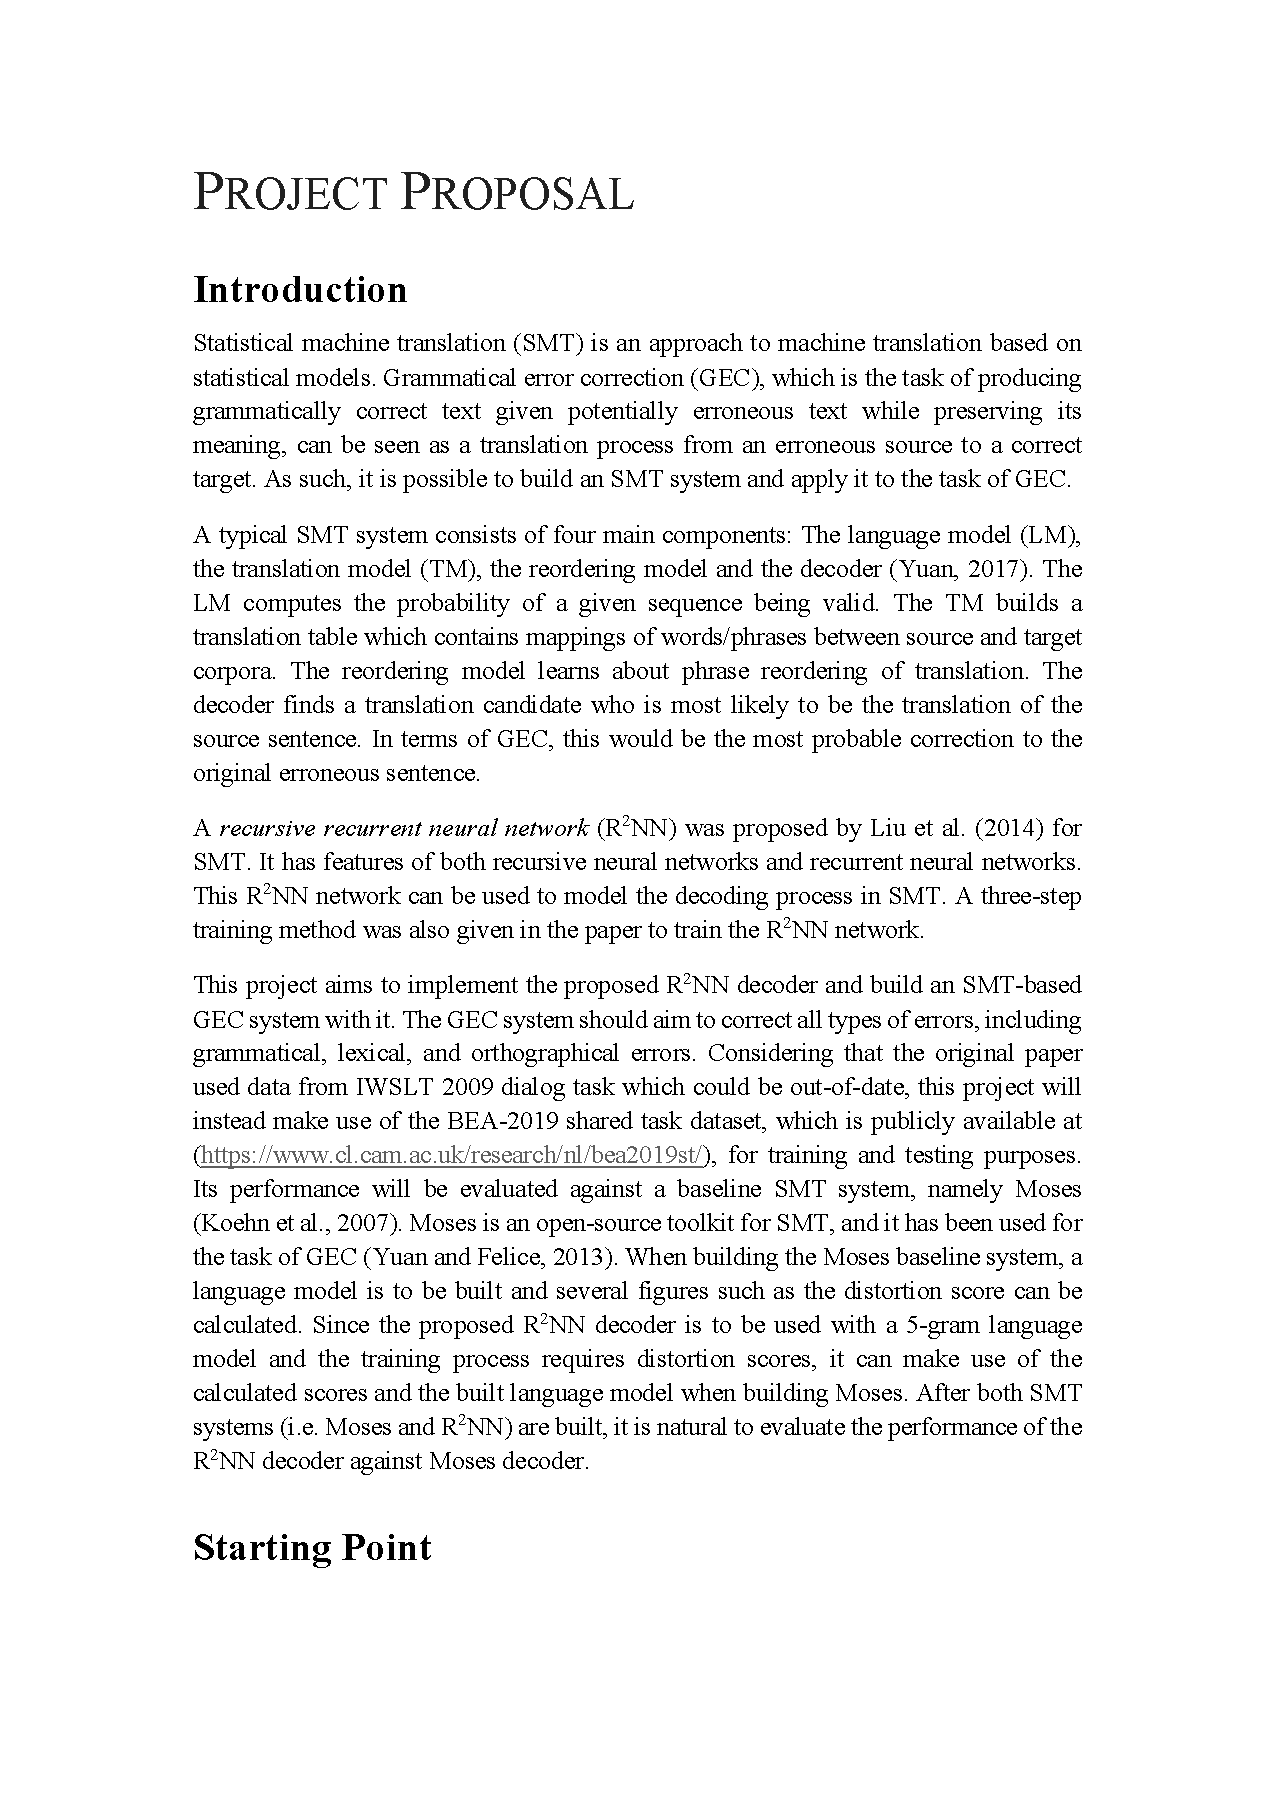
\includepdf[pages=-]{proposal.pdf}

% \chapter{Latex source}

% \section{diss.tex}
% {\scriptsize\lstinputlisting[language=TeX]{diss.tex}}

% \section{proposal.tex}
% {\scriptsize\verbatiminput{proposal.tex}}

% \chapter{Makefile}

% \section{refs.bib}
% {\scriptsize\verbatiminput{refs.bib}}


% \chapter{Project Proposal}

% \input{proposal}

\end{document}